\documentclass[a4,12pt]{article}
\usepackage{setspace}

%\usepackage{fullpage}
%\usepackage[top=1in, bottom=1in, left=1in, right=1in]{geometry}
\usepackage[margin=1in,paperwidth=8.5in,paperheight=11in,scale=0.75,bmargin=2.0cm,footnotesep=1cm]{geometry}
\usepackage{amsfonts,float,textcomp}
\usepackage{graphicx} %to include images
\usepackage[font={small}]{caption}
%\usepackage{apacite}
%\usepackage{natbib}
\usepackage[colorlinks=true, citecolor=blue]{hyperref}
\usepackage{hyperref}
\usepackage{xcolor}
\usepackage{url}
\usepackage{sidecap}
\usepackage{float}
\usepackage{caption}
\usepackage{multicol}
\usepackage{subcaption}
\usepackage[italic]{hepnames}
\usepackage{amssymb}
\usepackage{amsmath, mathtools}
\allowdisplaybreaks
%\linespread
%\usepackage{mciteplus}
\usepackage{listings}
\usepackage{mathtools}
\usepackage{physics}
\usepackage{braket}
\usepackage{gensymb}
\usepackage{slashed}
\usepackage[T1]{fontenc}
\usepackage[utf8]{inputenc}
\usepackage[backend=biber,style=numeric,autocite=plain,sorting=none]{biblatex}
\addbibresource{References.bib}
%\usepackage{nomencl}
\usepackage[nocfg]{nomencl}
\makenomenclature
\usepackage{setspace}
\usepackage{multirow}
\usepackage{empheq}
\usepackage{longtable}
\usepackage{chngcntr}
\counterwithin{figure}{section}
%\usepackage[backend=bibtex]{biblatex}
%\makenomenclature

\definecolor{codegreen}{rgb}{0,0.6,0}
\definecolor{codegray}{rgb}{0.5,0.5,0.5}
\definecolor{codepurple}{rgb}{0.58,0,0.82}
\definecolor{backcolour}{rgb}{0.95,0.95,0.92}

\lstdefinestyle{mystyle}{
    backgroundcolor=\color{backcolour},   
    commentstyle=\color{codegreen},
    keywordstyle=\color{magenta},
    numberstyle=\tiny\color{codegray},
    stringstyle=\color{codepurple},
    basicstyle=\ttfamily\footnotesize,
    breakatwhitespace=false,         
    breaklines=true,                 
    captionpos=b,                    
    keepspaces=true,                 
    numbers=left,                    
    numbersep=5pt,                  
    showspaces=false,                
    showstringspaces=false,
    showtabs=false,                  
    tabsize=2
}

\lstset{style=mystyle}






\usepackage{titlesec}
%\newcommand{\sectionbreak}{\clearpage}
\newcommand{\Lagr}{\mathcal{L}}
\numberwithin{equation}{subsection}
%\renewcommand{\nomname}{\centering List of Symbols}
\renewcommand*{\nompreamble}{\begin{multicols}{2}}
\renewcommand*{\nompostamble}{\end{multicols}}
\setlength{\columnsep}{3em}
\setlength{\nomitemsep}{0.02cm}
\usepackage[most]{tcolorbox}
\newtcolorbox{mybox}[2][breakable]{%
  attach boxed title to top center
               = {yshift=-8pt},
  colback      = blue!5!white,
  colframe     = blue!75!black,
  fonttitle    = \bfseries,
  colbacktitle = blue!85!black,
  title        = #2,#1,
  enhanced,
}
\newcommand\MTkillspecial[1]{% helper macro
\bgroup
\catcode`\&=9
\let\\\relax%
\scantokens{#1}%
\egroup
}
\DeclarePairedDelimiter\brkbraces\{\}
\reDeclarePairedDelimiterInnerWrapper\brkbraces{star}{
\mathopen{#1\vphantom{\MTkillspecial{#2}}\kern-\nulldelimiterspace\right.}
#2
\mathclose{\left.\kern-\nulldelimiterspace\vphantom{\MTkillspecial{#2}}#3}}
\usepackage[toc,page]{appendix}
\DeclareUnicodeCharacter{2009}{ }
\newcommand{\taninv}{\tan^{-1}}
\newcommand{\sininv}{\sin^{-1}}
\newcommand{\cosinv}{\cos^{-1}}

%\usepackage[scale=0.75,bmargin=1cm,footnotesep=1cm]{geometry}
%\usepackage[table]{xcolor}
%\usepackage{tabularx}
\setcounter{secnumdepth}{4}
\makeatletter
\setlength{\@fptop}{0pt}
\makeatother
\usepackage{atbegshi}% http://ctan.org/pkg/atbegshi
\AtBeginDocument{\AtBeginShipoutNext{\AtBeginShipoutDiscard}}
\onehalfspacing
\begin{document}
%\mbox{}
\begin{titlepage}
    \begin{center}
        \title{\textbf{Ph.D. Coursework Tutorial Report} \\ Errors and Uncertainties in Numerical Computations}
        \vspace{1.5cm}
        %\subtitle{Phenomenoloy of Neutrino Oscillations using Long Baseline Neutrino Experiments}
		\author{\textsc{\textbf{Ishwar Singh}}\\ \\ \textit{ Submitted to:} \textsc{\textbf{Prof. Awadesh Prasad}}}
		\vspace{0.7cm}
		\date{\today}
		\maketitle
		\thispagestyle{empty}
				\begin{figure}[H]
				\begin{center}
        
\includegraphics[scale=0.4]{University_of_delhi_logo.png}
				\end{center}
				\end{figure}
       	\vspace{0.8cm}
       	\begin{center}
        Department of Physics and Astrophysics\\
        University of Delhi\\
        New Delhi, India\\
				\end{center}


    \end{center}
\end{titlepage}
\printnomenclature[3em]
\tableofcontents
\thispagestyle{empty}
\listoffigures
%\listoftables
\thispagestyle{empty}
%\mbox
\newpage
\clearpage
\pagebreak
\setcounter{page}{1}

\section{Introduction}
Recently, a new category, computational physics, has been added to the traditional physics classification scheme. This new category acts as a bridge between the traditional theoretical and experimental physics. Computer simulations have become an integral part of not only every branch of physics but also in other disciplines of science. With each advancement of computer technology, the usage of computers for scientific computation has also increased substantially.\\
\newline
Although, computers are very powerful, but they have limitations. The representation of real numbers in computers is one of the most import limitations of computers. The computer is a finite system. This inability of the computers i.e. to store `exact' real numbers, gives rise to the errors in floating point computations.\\
\newline
These errors, although small ($ \epsilon \approx 10^{-7}$ for single precision and $ \epsilon \approx 10^{-15}$ for double precision), propagates after every usage, might lead to unexpected results (known as garbage values). Therefore, it is imperative to study the errors involved in scientific computations before actually jumping into the field which requires computations.

\section{Representation of Numbers in Computers}
Computers are binary machines i.e. they understands sequences of binary integers (known as bits) i.e. zeros (0's) and ones (1's). All computations are also done using these arrays of zeros (0's) and ones (1's). These long arrays of binary digits are good only for computers, but it is not user friendly. A user enters his data in decimal numbers and expects his answer in decimal numbers only. A group  of these bits is collectively known as a word with a well defined length. The computers are very fluent in this (binary numbers) mode of communication. Different computers might have different word lengths, but this length is generally expressed in bytes, with 

$$1 \text{ byte} \equiv 1 \text{B} = 8 \text{ bits}.$$
\newline
This seems a right time to introduce the single precision and double precision numbers. A single precision number is stored in an array of 32-bits i.e. 4 bytes, while the double precision number is stored in an array of 64-bits are 8 bytes. These two terms will reoccur multiple times in this report.\\

 \subsection{Integers}
 It is easier for computers to deal with the integers. In total 32 bits are allotted to store the integers, out of which 31 bits stores a straight binary number and 1 bit is for sign. The largest number which can be store is,
 $$(01111.....1111)_2 = 2^{31}-1 = 2,147,483,647.$$ 

 \subsection{Real Numbers}
 Storing real numbers is a bit complex. There exists two possible ways of storing real numbers in computers : (i) \textit{fixed point representation} and (ii) \textit{floating point representation}. In the fixed point representation methods, a fix number of bits are reserved before and after the decimal point. This method was good for example banking system where 2 or 3 numbers are required after the decimal point, but wasn't good for scientific purposes. The floating point method is used for scientific computations. \\
 \newline
 In general, a fractional number, of precision $p$, base $\beta$ and exponent $e$, is represented as, 

 $$\pm d_0.d_1d_2d_3.....d_{p-1} \times \beta^e,$$
 which has the value,
 $$\pm (d_0 + d_1 \beta^{-1} + d_2 \beta^{-2}+.......+ d_{p-1} \beta^{-(p-1)})\beta^e.$$
 The numbers before the base $\beta$, i.e. $\pm d_0.d_1d_2d_3.....d_{p-1}$  is known as the mantissa. For computers the base is fixed i.e. $\beta=2$. The mantissa and exponents, depending upon the precision requires for a computation, are allotted different finite numbers of bits. In a single precision number (32-bits) the mantissa carries 23 bits, the exponent carries 8 bits and 1 bit is reserved for sign of the number. In a double precision number (64-bits), the mantissa carries 53 bits, the exponent carries 11 bits. Please note that in both cases the numbers of bits assigned to the manstissa and the exponent is finite. Generally, a bias is added in the exponent. The single precision floats have a bias of + 127. Therefore, the stored exponent is = true exponent + 127.\\
 \newline
 The IEEE standard also reserves some special arrangements of mantissa and exponents for special values like $\pm \infty$ and for NaN (not a number). Exponent 255 is reserved for these special values. Table \ref{tab:tabel1} shows few relevant specifications of single-precision and double-precision data types.

\begin{table}[h]
\centering
\begin{tabular}{|l|l|l|}
\hline
         & \textbf{float}                         & \textbf{double}                         \\
         \hline
\textbf{bits}     & 32                                     & 64                                      \\
\textbf{bytes}    & 4                                      & 8                                       \\
\textbf{range}    & $\approx 10^{-38} \text{ to } 10^{38}$ & $ \approx 10^{-38} \text{ to } 10^{38}$ \\
\textbf{accuracy} & 7 decimals                             & 16 decimals \\
\hline                           
\end{tabular}
\caption{Specifications of single-precision (float) and double-precision (double) data types.}
\label{tab:tabel1}
\end{table}

\section{Types of Errors}
Every measurement is prone to errors. Sometimes these errors are caused by the researcher's negligence, some measurement are prone to random errors. Similarly, some errors are introduced by the computers used to perform a scientific computations. This section will deal with different types of errors and uncertainties introduced due to computer computations.
\newline
Let's assume that a computation task is finished after $n$ complex loops or steps. Let $p$ be the probability of success of each step, then the joint probability of the complete program/code is $P=p^{n}$. If $p = 0.9993$ i.e. very likely to be true, after $n=1000$ steps, the probability of the code to return correct result is $P \approx \frac{1}{2}$ i.e. the result is equally likely to give garbage values (wrong results). The most dominant errors in floating point computations are discussed in the upcoming sections.

\subsection{Bad Theory or Blunders}
These errors are introduced due to typographical errors which might cause syntax errors in the codes, running a different program or having a fault in the reasoning behind the code, using data which has errors in itself which is not known to the programmer. These errors can only be resolved by the programmer itself. One of the best ways to avoid such errors is to verify if the code is doing what the programmer every now and then.

\subsection{Random Errors}
These errors are caused by random events such as fluctuations in electronic components of the system, cosmic ray interactions inside the system (very very unlikely though) or if someone pulls the plug of your system and the system shuts down. All these errors are very unlikely for small codes or programs. But these errors might be relevant for a week long simulations. This error is irrelevant for this project.

\subsection{Round-off Errors}
A finite number of bits is available with the computer (23 bits for single precision and 53 bits for double precision data types) to store the mantissa of any number stored in it. The float data type can hold numbers up to 7 significant figure while the double data type can hold up to 16 significant numbers. If a float type variable is asked to store a number with 10 significant digits, computer will store a rounded-off 7 significant digit number in it's memory. The same happen with the double data type \footnote[1]{If the significant digits of number is greater than 16.}. This rounding off the numbers introduces errors in the computations which grows up with each arithmetic operation. The computer stores an exact number `$a$' is stored as `$a_c$' such that 
$$a_c = a(1+\epsilon_a),$$
where $\epsilon_a$ is the relative round off error in $a$. 

\subsubsection{Round-off Error in a Single Step}
Division of two numbers, as calculated by the computer is given as,

\begin{align}
a=\frac{b}{c} & \Rightarrow a_c = \frac{b_c}{c_c} = \frac{b(1+\epsilon_b)}{c(1+\epsilon_c)} && \\
& \Rightarrow \frac{a_c}{a} = \frac{1+\epsilon_b}{1+\epsilon_c} \approx (1+\epsilon_b)(1-\epsilon_c) \approx 1+ \epsilon_b - \epsilon_c &&\\
& \Rightarrow \frac{a_c}{a} \approx 1 + |\epsilon_b| + |\epsilon_c| &&
\end{align}
Notice however that in the above derivation very small $\epsilon^2$ term has been ignored and the modulus is used to find the maximum error in the calculation. Note also that this is the basic error propagation rule which we use in our laboratory calculations.

\subsubsection{Round-off Error Propagation After N Steps}
As we have seen in the previous section, the round-off error accumulates after each calculational step. In general, If there are $N$ calculational steps involved in an algorithm, the total relative error $\epsilon_{ro}$ becomes,

$$\epsilon_{ro} \simeq \sqrt N \epsilon_m.$$
where $\epsilon_m$ is the machine epsilon. Machine epsilon is the minimum number such that a system can differentiate $1.0$ from $1.0+\epsilon_m$. In other words,

$$1.0 + \epsilon_m > 1.0.$$
 This is equivalent to the least count of any apparatus we use in our laboratory. This $\epsilon_m \simeq 10^{-7}$ and $\epsilon_m \simeq 10^{-16}$ for float and double data type respectively. Machine epsilon plays an important role in defining errors in scientific computations. This machine epsilon is the upper bound of the round off errors.
\newline
The fact that round-off errors accumulates with each computational steps, makes it necessary to study the variation of these errors with N. This helps the programmer to figure out when to stop the iteration.

\subsubsection{Subtractive Cancellation}
This is actually an arithmetic error which arises if two large and approximately equal numbers are subtracted, the relative error in the answer increases after each step. Consider the subtraction of two numbers,

\begin{align}
a = b - c & \Rightarrow a_c \simeq b_c - c_c \simeq b(1+\epsilon_b) - c(1+\epsilon_c) && \\
& \Rightarrow \frac{a_c}{a} \simeq 1+ \epsilon_b \frac{b}{a} - \epsilon_c \frac{c}{a} .&&
\end{align}
It can be observed very clearly that if both the numbers are approximately same i.e. $a \simeq b$, relative error in a becomes,

\begin{equation}
  \frac{a_c}{a} = 1 + \epsilon_a \simeq 1+ \frac{b}{a}(\epsilon_b-\epsilon_c) \simeq 1+\frac{b}{a} \text{max}(|\epsilon_b|, |\epsilon_c|)
\end{equation}
Although the relative errors in $b$ and $c$ are subtracted, but final relative error is multiplied by a large factor $\frac{b}{a}$ which ultimately magnifies the error.

\subsubsection{Implementation and Assessment }
\paragraph{Machine Epsilon:}
Listing \ref{list1} shows the code used calculate the machine epsilon of double data types. The output gives the value of machine error as $2.22045e-16$. A similar code was run to calculate the machine epsilon for float data type, which was found out to be $1.19209e-07$.  

\begin{lstlisting}[language=C++, caption= Code to calculate the machine epsilon of double data types., label= list1]
#include<iostream>
#include <cfloat>
using namespace std;

// Function for Machine Epsilon with an
// initial value provided as EPS.
void machineEpsilon(double EPS)
{
    // taking a floating type variable
    double prev_epsilon;

    // run until condition satisfy
    while ((1+EPS) != 1)
    {
        // copying value of epsilon into previous epsilon
        prev_epsilon = EPS;

        // dividing epsilon by 2
        EPS /=2;
    }

    // print output of the program
    cout << "Machine Epsilon is : " << prev_epsilon << endl;
}
// Driver Code
int main()
{
    // calling function which calculate machine epsilon
    // with initial value provided as 0.5
    machineEpsilon(0.5);

    return 0;
}
\end{lstlisting}

\paragraph{Series Sum : } Subtractive cancellation is a dominant source of errors in the sum of a series containing alternative signs. Consider for an example , a finite series,
\begin{equation}
S^{(1)}_N = \sum_{n=1}^{2N} (-1)^n \frac{n}{n+1}.
\end{equation}
The above sum can be divided into even and odd values of $n$ separately, which gives,

\begin{equation}
S^{(2)}_N = - \sum_{n=1}^{N} \frac{2n-1}{2n} + \sum_{n=1}^{N}\frac{2n}{2n+1}.
\end{equation}
Sum $S^{(2)}_N$ involves only subtraction of two series (without any alternative sign). Even this single subtraction might cause sufficient subtractive cancellation. Even this single subtraction can be avoided if the sum is written as 

\begin{equation}
S^{(3)}_N = \sum_{n=1}^{N} \frac{1}{2n(2n+1)}.
\end{equation}
Mathematically all of these sums i.e. $S^{(1)}_N$, $S^{(2)}_N$ and $S^{(3)}_N$ are equal, but they might give different numerical results. Listing \ref{list2} lists a C++ code to calculate $\text{log}_{10}|(S^{(1)}_N-S^{(3)}_N)/S^{(3)}_N|$ as a function of $\text{log}_{10}(N)$.

\begin{lstlisting}[language=C++, caption= C++ code to calculate $\text{log}_{10}|(S^{(1)}_N-S^{(3)}_N)/S^{(3)}_N|$ as a function of $\text{log}_{10}(N)$., label= list2]
/*
Name  - Ishwar Singh
Aim   - Error analysis in series sum.
Email - ishwarsaini10@gmail.com
*/

/*C++ Directives*/
#include<iostream>
#include<stdio.h>
#include<math.h>
#include<iomanip>
#include<fstream>


float series1(int n){
    int   i ;
    float t ;
    float s ;
    s = t = -1.0/2.0  ;
    for(i=1;  i<2*n;  i++){
        t*=-(pow((i+1),2))/(i*(i+2))  ;
        s+=t;
    }
    return(s);
}

float series2(int n){
    int   i   ;
    float t1  ;
    float t2  ;
    float s1  ;
    float s2  ;
    s1  = t1  = 1.0/2.0   ;
    s2  = t2  = 2.0/3.0   ;
    for(i=1;  i<n;  i++){
        t1*=((2*i+1)*i)/((2*n-1)*(n+1))       ;
        t2*=((2*i+2)*(2*i+1))/((2*i+3)*(2*i)) ;
        s1+=t1;
        s2+=t2;
    }
    return(s2-s1);
}

float series3(int n){
    int   i ;
    float t ;
    float s ;
    s = t = 1.0/6.0  ;
    for(i=1;  i<n;  i++){
        t*=(n*(2*n+1))/((n+1)*(2*n+3));
        s+=t;
    }
    return(s);
}
int main(){
    int N;
    float s1_final  ;
    float s2_final  ;
    float s3_final  ;
    std::ofstream myfile;
    myfile.open("series1.dat");
    std::cout <<  std::setprecision(7) << std::setw(10) ;

    for(int N=1;  N<=100; N++){
        s1_final  = series1(N);
        s2_final  = series2(N);
        s3_final  = series3(N);
        myfile <<  log10(N)  <<  "\t"  <<  log10(abs((s1_final-s3_final)/s3_final))  <<  std::endl;
    }
    myfile.close();
    return 0;
}
\end{lstlisting}
Figure \ref{series_sum} shows the variation of $\text{log}_{10}|(S^{(1)}_N-S^{(3)}_N)/S^{(3)}_N|$ as a function of $\text{log}_{10}(N)$. The following observations can be made by analyzing this plot : 

  \begin{itemize}
     \item[--] Negative of the ordinate gives the number of significant figures used in the calculation. This variation of negative ordinate shows the loss of significance of the answer.
     \item[--] There is a linear variation in the initial part of the plot which shows that the error due to subtractive cancellation is proportional to a power of $N$.
  \end{itemize}  



\begin{figure}[h]
    \centering
    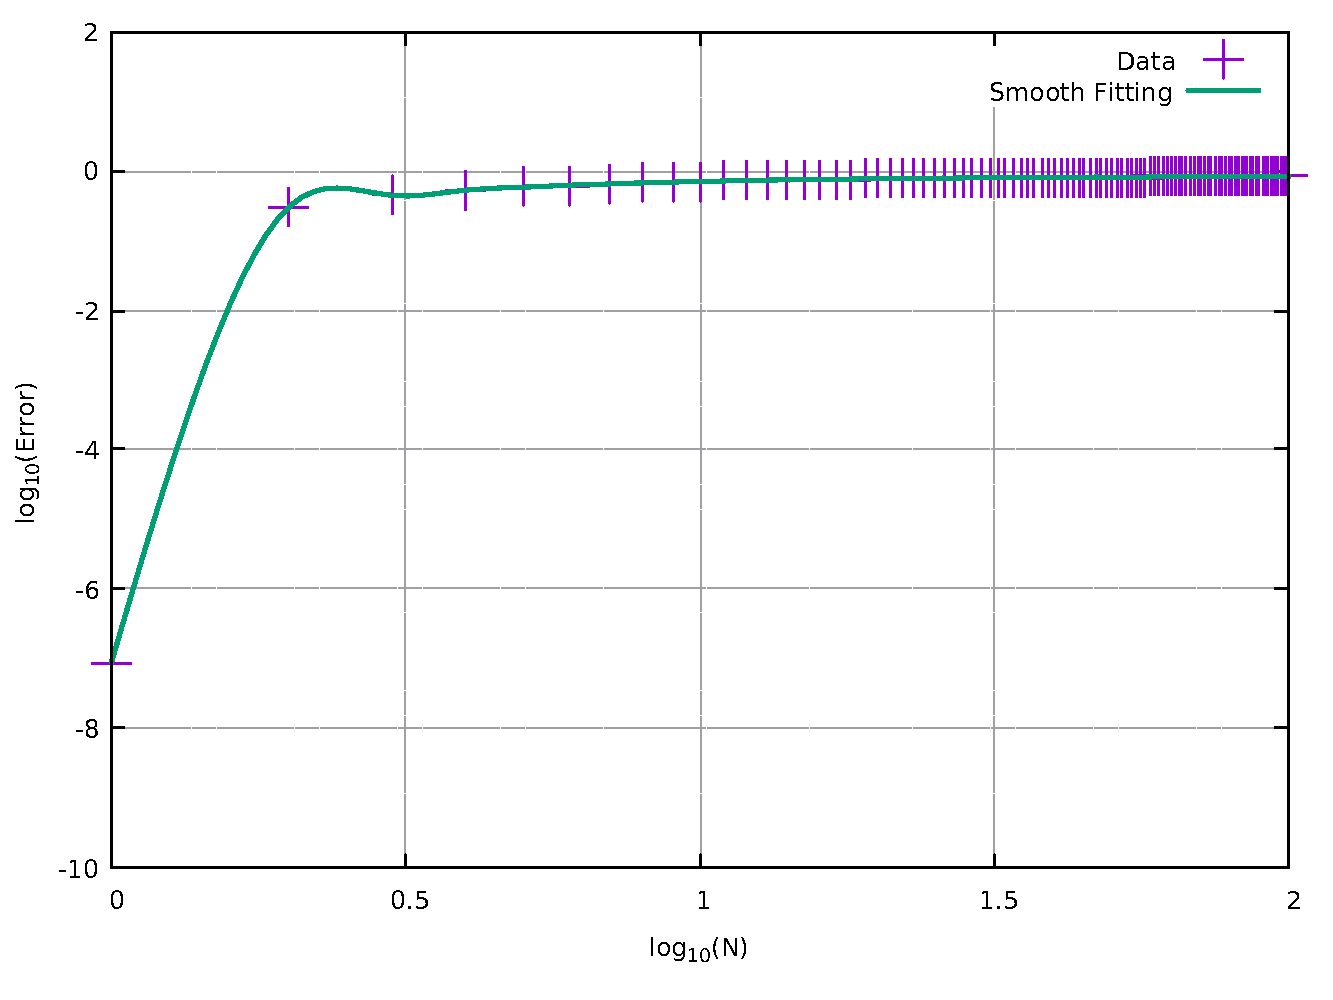
\includegraphics[height=7.0cm, width=11.0cm]{/home/ishwarsingh/Phd_Documents/Course_work/Tutorial/Report/Images/Errors_in_series_sum_06-11-2020_v2.pdf}
  \caption{Variation of $\text{log}_{10}|(S^{(1)}_N-S^{(3)}_N)/S^{(3)}_N|$ as a function of $\text{log}_{10}(N)$.}
  \label{series_sum}
\end{figure}

\paragraph{Errors in Spherical Bessel Functions: } Spherical Bessel functions are actually solutions of the differential equation,

\begin{equation}
  x^2 f^{\prime\prime}(x)+ 2x f^{\prime}(x)+[x^2-l(l+1)]f(x)=0.
\end{equation}
There are various methods to calculate the values of these functions. One of the methods is the numerical recursion relations method. These recursion relations can be used both ways i.e. upward recursion relation and downward recursion relations

\begin{equation}
  j_{l+1} = \frac{2l+1}{x}j_l(x) - j_{l-1}(x), \text{ (up)}
\end{equation}

\begin{equation}
  j_{l-1} = \frac{2l+1}{x}j_l(x) - j_{l+1}(x) \text{ (down).}
\end{equation}

\begin{lstlisting}[language=C++, caption= C++ code to calculate the Bessel functions using upward and downward recursion relations and the associated errors., label= list2]
/*
 * Name - Ishwar Singh
 * Aim  - To calculate the values and errors in Bessels functions using recursion relations.
 * Date - 08.11.2020
 * Emai - isingh@fnal.gov
*/
// C++ Directives
#include<iostream>
#include<stdio.h>
#include<math.h>
#include<cfloat>
#include<iomanip>
#include<fstream>

float bessels_up (float x, int l){
    int s = 25  ;
    float a  = sin(x)/x ;
    float b  = (sin(x)/pow(x,2))-cos(x)/x ;
    float j[s]  = {a,b}  ;
    for(int k = 1;  k<s-1;  k++){
        j[k+1]  = ((2*k+1)/x)*j[k]-j[k-1];
    }
    //float scale = (sin(x)/x)/j[0]; 
    return j[l] ;
}

float bessels_down (float x, int l){
    int s = 25  ;
    float j[s]  = {}  ;
          j[23] = 1.0 ;
          j[24] = 1.0 ;
    for(int k = s-2;  k>0;  k--){
        j[k-1]  = ((2*k+1)/x)*j[k]-j[k+1];
    }
    float scale = (sin(x)/x)/j[0]; 
    return j[l]*scale ;
}
int main(){
    float x ;
    int i   ;
    std::ofstream my_file;
    my_file.open("Bessels.txt");
    for(int i =  0;  i<=25;  i++){
        x = 1.0;
        my_file <<  std::fixed  <<  std::setprecision(7)  <<  i <<  "\t"  <<  bessels_up(x,i) <<  "\t"  <<  bessels_down(x,i) <<  "\t"  << abs(bessels_up(x,i)-bessels_down(x,i))/(abs(bessels_up(x,i))+abs(bessels_down(x,i))) <<    std::endl;
    }

    return 0;
}
\end{lstlisting}

\begin{figure}[h]
    \centering
    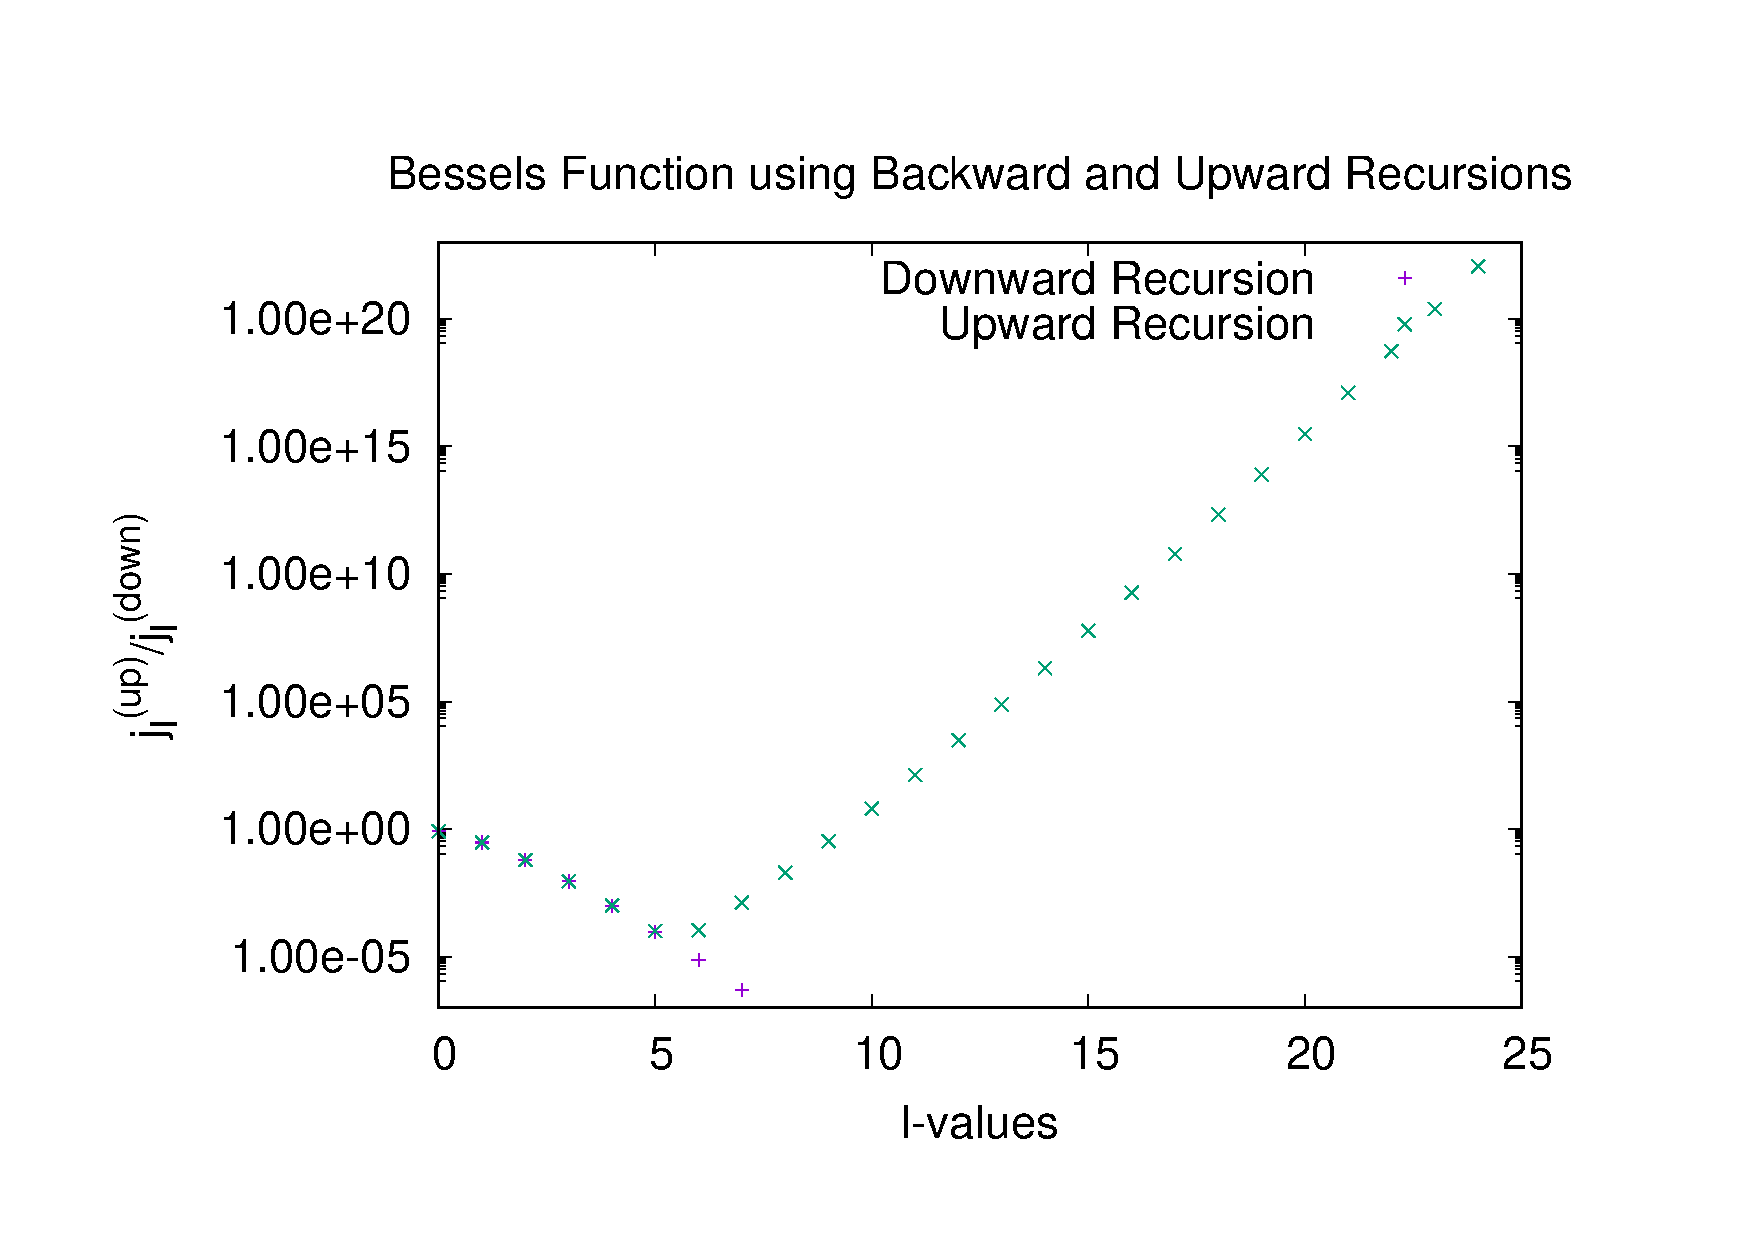
\includegraphics[scale=0.5]{/home/ishwarsingh/Phd_Documents/Course_work/Tutorial/Report/Images/bessels_v1.pdf}
  \caption{Bessel functions using upward and downward recursion relations.}
  \label{fig:bessel_v1}
\end{figure}


\begin{figure}[h]
    \centering
    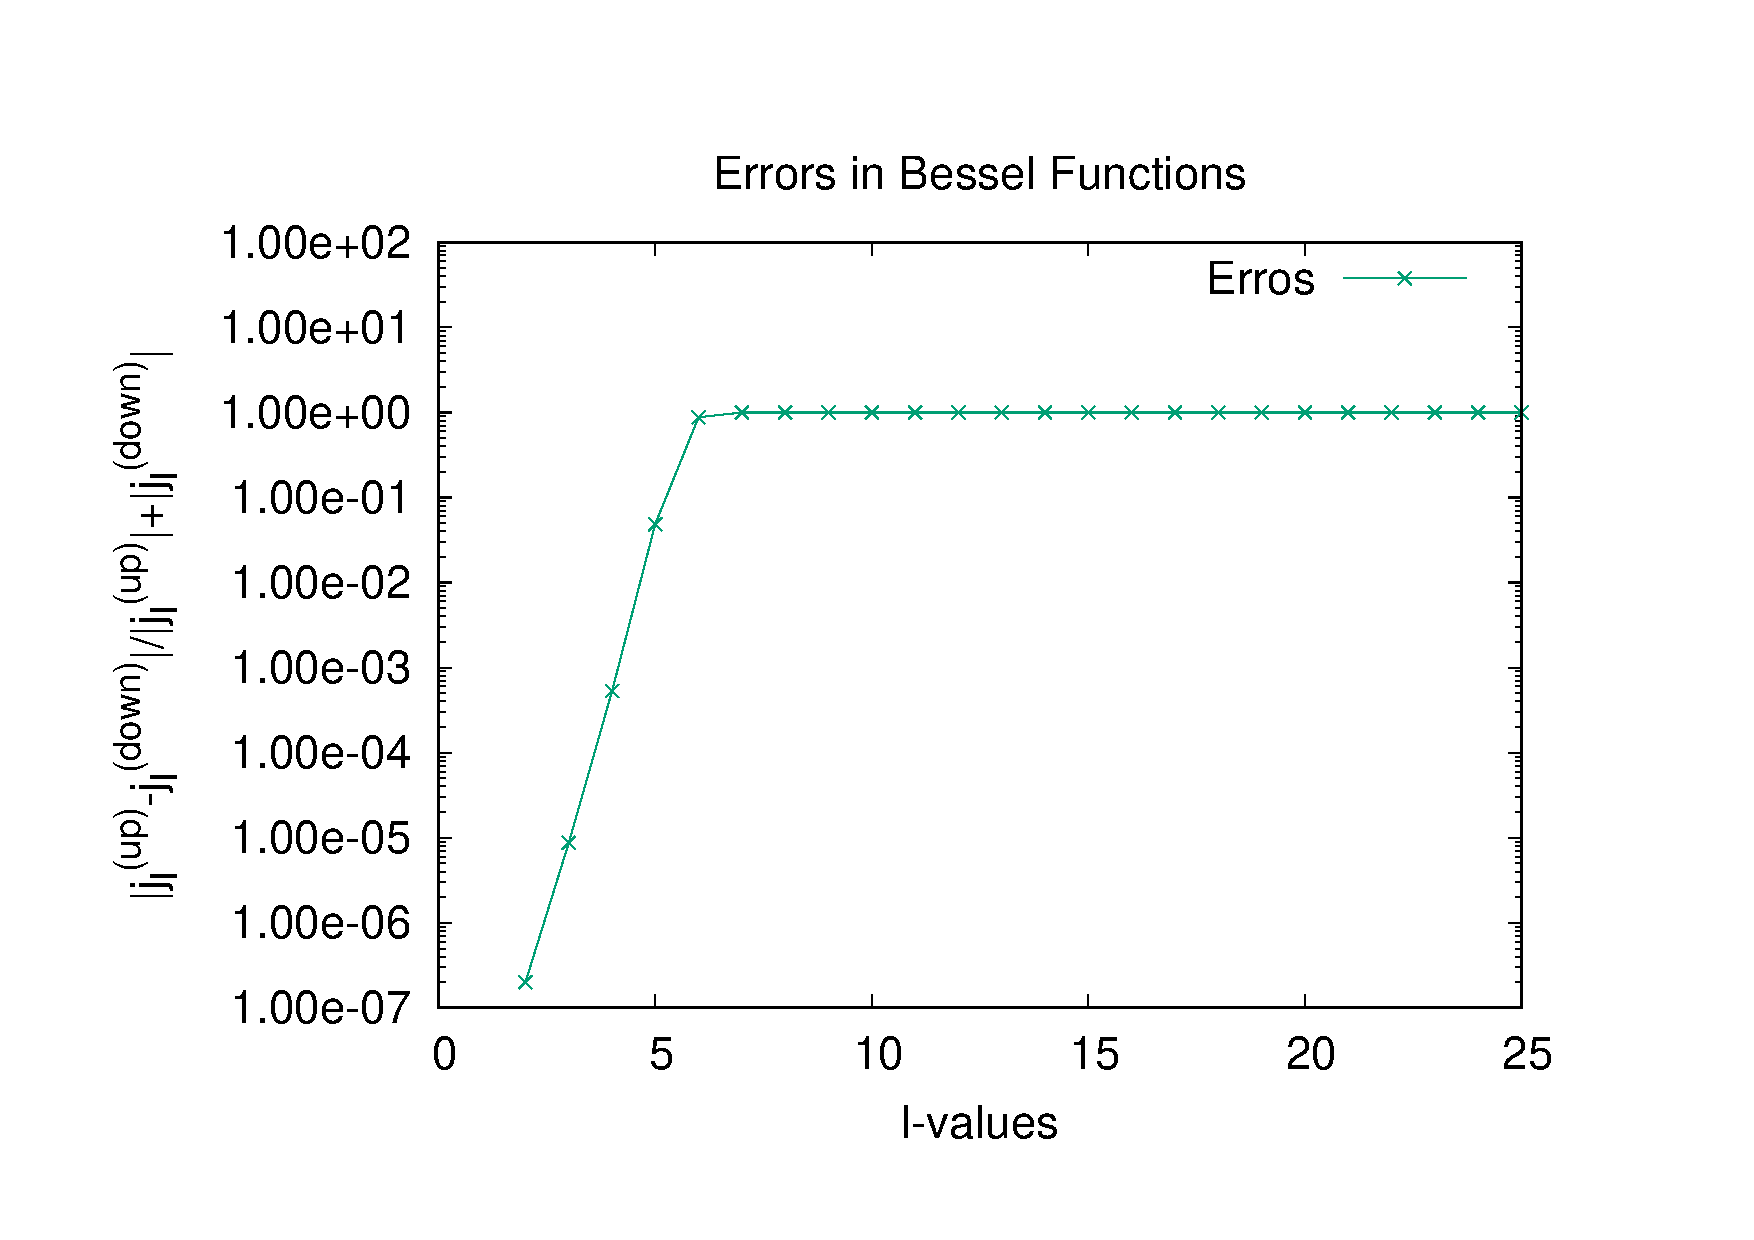
\includegraphics[scale=0.5]{/home/ishwarsingh/Phd_Documents/Course_work/Tutorial/Report/Images/bessels_v2.pdf}
  \caption{Subtractive cancellation errors in Bessel functions.}
  \label{fig:bessel_v2}
\end{figure}

%\begin{mybox}[colback=white, breakable]{Code to Find Machine Epsilon}
%\lstinputlisting[language=C++]{/home/ishwarsingh/Phd_Documents/Course_work/Tutorial/Report/Codes/MEPS.cpp}
%\end{mybox}b

\textbf{Observations : }
  \begin{itemize}
    \item Figure \ref{fig:bessel_v1} shows that both the upward and downward recursion methods converge in some region of the plot. After $l=5$, the upward recursion begins to diverge because of the fact that in the upward recursion method, two large numbers are subtracted to give small numbers and hence subtractive cancellation is present. However, this is not the case with downward recursion relation.

    \item Figure \ref{fig:bessel_v2} shows the variation of subtractive cancellation errors in Bessel function. The linear variation shows that the error varies as power of $l$. 
  \end{itemize}

\paragraph{Iterative Addition : } This is yet another example of propagation of round-off errors after each calculation step. The algorithm used is,
$$x_{n+1}= x_n + dx$$ 
The C++ code simply calculates the final answer for a given $x_n$, $dx$ for a fixed value of $n=10^6$ and compares the numerical answer with the actual answer.

 \begin{lstlisting}[language=C++, caption= C++ code to implement iterative addition algorithm., label= list3]
#include<iostream>
#include<stdio.h>
#include<math.h>
#include<cfloat>
#include<iomanip>
#include<fstream>

void iterative_addition(float x, float dx, float true_val){
    float temp  = x ;
    for (int i=1;i<=10E6;i++){
        x+=dx;
    }
    std::cout <<  temp  <<  "\t"  <<  dx  <<  "\t" << x <<  "\t"  << abs((true_val-x)/true_val) <<     std::endl;
}

int main(){
    float x1  = 0.1 ;
    float dx1 = 0.1 ;
    float x2  = 0.01  ;
    float dx2 = 0.01  ;
    float x3  = 0.001 ;
    float dx3 = 0.001 ;
    float x4  = 1E-7  ;
    float dx4 = 1.0E-7;  
    iterative_addition(x1,dx1,  10E5);
    iterative_addition(x2,dx2,  10E4);
    iterative_addition(x3,dx3,  10E3);
    iterative_addition(x4,dx4,  10E-1);

    return 0;
}
\end{lstlisting} 

\begin{table}[h]
\centering
\begin{tabular}{|l|l|l|l|l|}
\hline
\textbf{x} & \textbf{dx} & \textbf{Numerical Value} & \textbf{True Value} & \textbf{Relative Error} \\
\hline
0.1        & 0.1         & 1.0879E+06               & 10E+5               & 0.0879371               \\
0.01       & 0.01        & 95681                    & 10E+4               & 0.0431905               \\
0.001      & 0.001       & 9780.21                  & 10E+3               & 0.0219795               \\
1E-7       & 1E-7        & 1.06477                  & 10E-1               & 0.0647676 \\
\hline             
\end{tabular}
\caption{Comparison of true and numerical values of iterative addition.}
\label{tab:my-table}
\end{table}

\subsection{Approximation Errors}
Consider we will have to use $\sin(x)$ in our program. Most of programming languages provides an in-built function which returns the values of such trigonometric functions. Mathematically these functions are actually an infinite series e.g. 
$$\sin(x) = \sum^{\infty}_{n=1} \frac{(-1)^{n-1}x^{2n-1}}{(2n-1)!} (\text{ exact }).$$
But it is not possible to compute all the terms in these functions. Most of the algorithms compute these sums to a finite number of terms i.e.
\begin{align}
\sin(x) &\approx \sum^{N}_{n=1} \frac{(-1)^{n-1}x^{2n-1}}{(2n-1)!} (\text{ algorithm }), && \\
        &= sin(x)+\epsilon(x,N), && 
 \end{align}  
 where $\epsilon(x,N)$ is known as the \textit{approximation error} which is given as,
$$\epsilon(x,N) = \sum^{\infty}_{N+1} \frac{(-1)^{n-1}x^{2n-1}}{(2n-1)!} .$$
As these errors arise from the algorithms used to approximate the mathematics, these errors are also known as \textit{algorithmic errors}. It seems reasonable to say that approximation errors decreases with the increasing value of $N$ and vanish in the limit where $N \to \infty$. In general, the approximation errors, $\epsilon_{approx}$, varies as, 
$$\epsilon_{approx} = \frac{\alpha}{N^{\beta}}.$$
where $\alpha$ and $\beta$ are arbitrary constants.

\subsubsection{General Algorithm to Compute Errors}
In a traditional physics laboratory experiment, the true value of the physical quantity measure in an experiment is generally known to us and hence error computation is a bit easier. However, this is not the case in a scientific computation. Therefore, some special techniques are utilized to calculate errors at each computational step. Let's assume $\mathcal{A}$ is the true value of any variable, if $A(N)$ is value of that variable after $N$ computational steps, then,
$$A(N) \simeq \mathcal{A} + \frac{\alpha}{N^{\beta}}.$$
One of the techniques to find the errors after each computational steps is to compute,
$$A(2N)-A(N) \simeq \frac{\alpha}{N^{\beta}},$$
and then plotting $\text{log}_{10}\left|[A(N)-A(2N)]/A(2N) \right|$ as a function of $\text{log}_{10}N$. This plot helps the programmer to determine the convergence of the algorithm.

\subsubsection{Implementation and Assessment}
\paragraph{Errors in $\sin(x)$ Series : } The Taylor series expansion of $\sin(x)$ is given as,

$$\sin(x)=\sum_{n=1}^{\infty} \frac{(-1)^{n-1} x^{2n-1}}{(2n-1)!}$$
Listing \ref{list5} lists a C++ code to calculate the approximation errors in the series sum which calculates errors as function of $N$ for various values of $x$.

\begin{lstlisting}[language=C++, caption= C++ code to calculate the approximation errors in the series sum of $\sin(x)$., label= list5]
/*
 * Name - Ishwar Singh
 * Aim  - To calculate the errors in sin sum series for different values of x.
 * Email  - isingh@fnal.gov
 * Date - 07.11.2020
 */

//  C++ Directives

#include<iostream>
#include<stdio.h>
#include<math.h>
#include<cfloat>
#include<iomanip>
#include<fstream>

/*  Function to find sum of sin series for a given and number of terms to be added  */
float sin_series(int N, float x){
    float s   ;
    float t   ;
    s = t = x ;
    for(int i=1;  i<N;  i++){
        t*=-x*x/((2*i+1)*2*i);
        s+=t;
    } 
    return s;
}

/*  Main function starts here */
int main(){
    std::ofstream my_file                   ; /*  Output file stream */
    std::string ini = "sin_series_file_v2_" ; 
    std::string txt = ".txt"                ;
    int i=1                                 ;
    for(int i=1;  i<=100;  i+=5){
        std::string final_name  = ini + std::to_string(i) + txt;
        std::ofstream my_file1              ;
        my_file1.open(final_name)           ;
        float x = i                         ;
        std::cout <<  std::fixed            ;
        std::cout <<  std::setprecision(7)  <<  x <<  std::endl ;
        for (int i=1; i<=100;  i++){
            my_file <<  std::setprecision(7)  <<  i <<  "\t"  <<  abs(sin_series(i,x)-sin_series(2*i,x)) <<  std::endl;
            my_file1 <<  std::setprecision(7)  <<  i <<  "\t"  <<  abs(sin_series(i,x)-sin_series(2*i,x)) <<  std::endl;
        }
    }
    return(0);
}
\end{lstlisting} 

\begin{figure}[h]
    \centering
    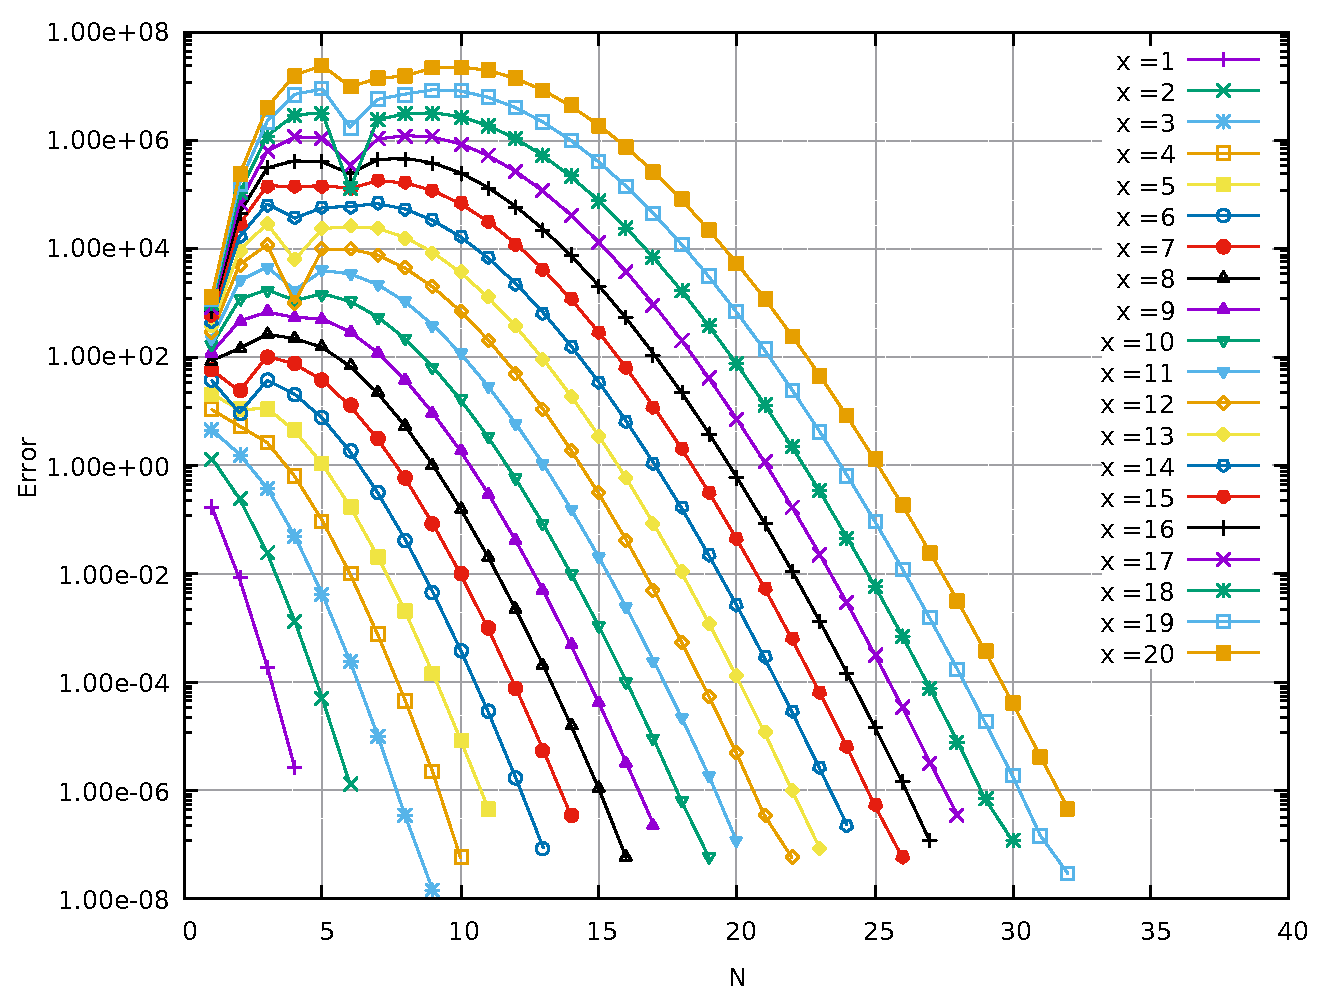
\includegraphics[scale=0.5]{/home/ishwarsingh/Phd_Documents/Course_work/Tutorial/Report/Images/sin_series_error_v1.pdf}
  \caption{Approximation errors in series sum of $\sin(x)$ for $x=1$ to $x=20$.}
  \label{fig:sin_series_error1}
\end{figure}

\begin{figure}[h]
    \centering
    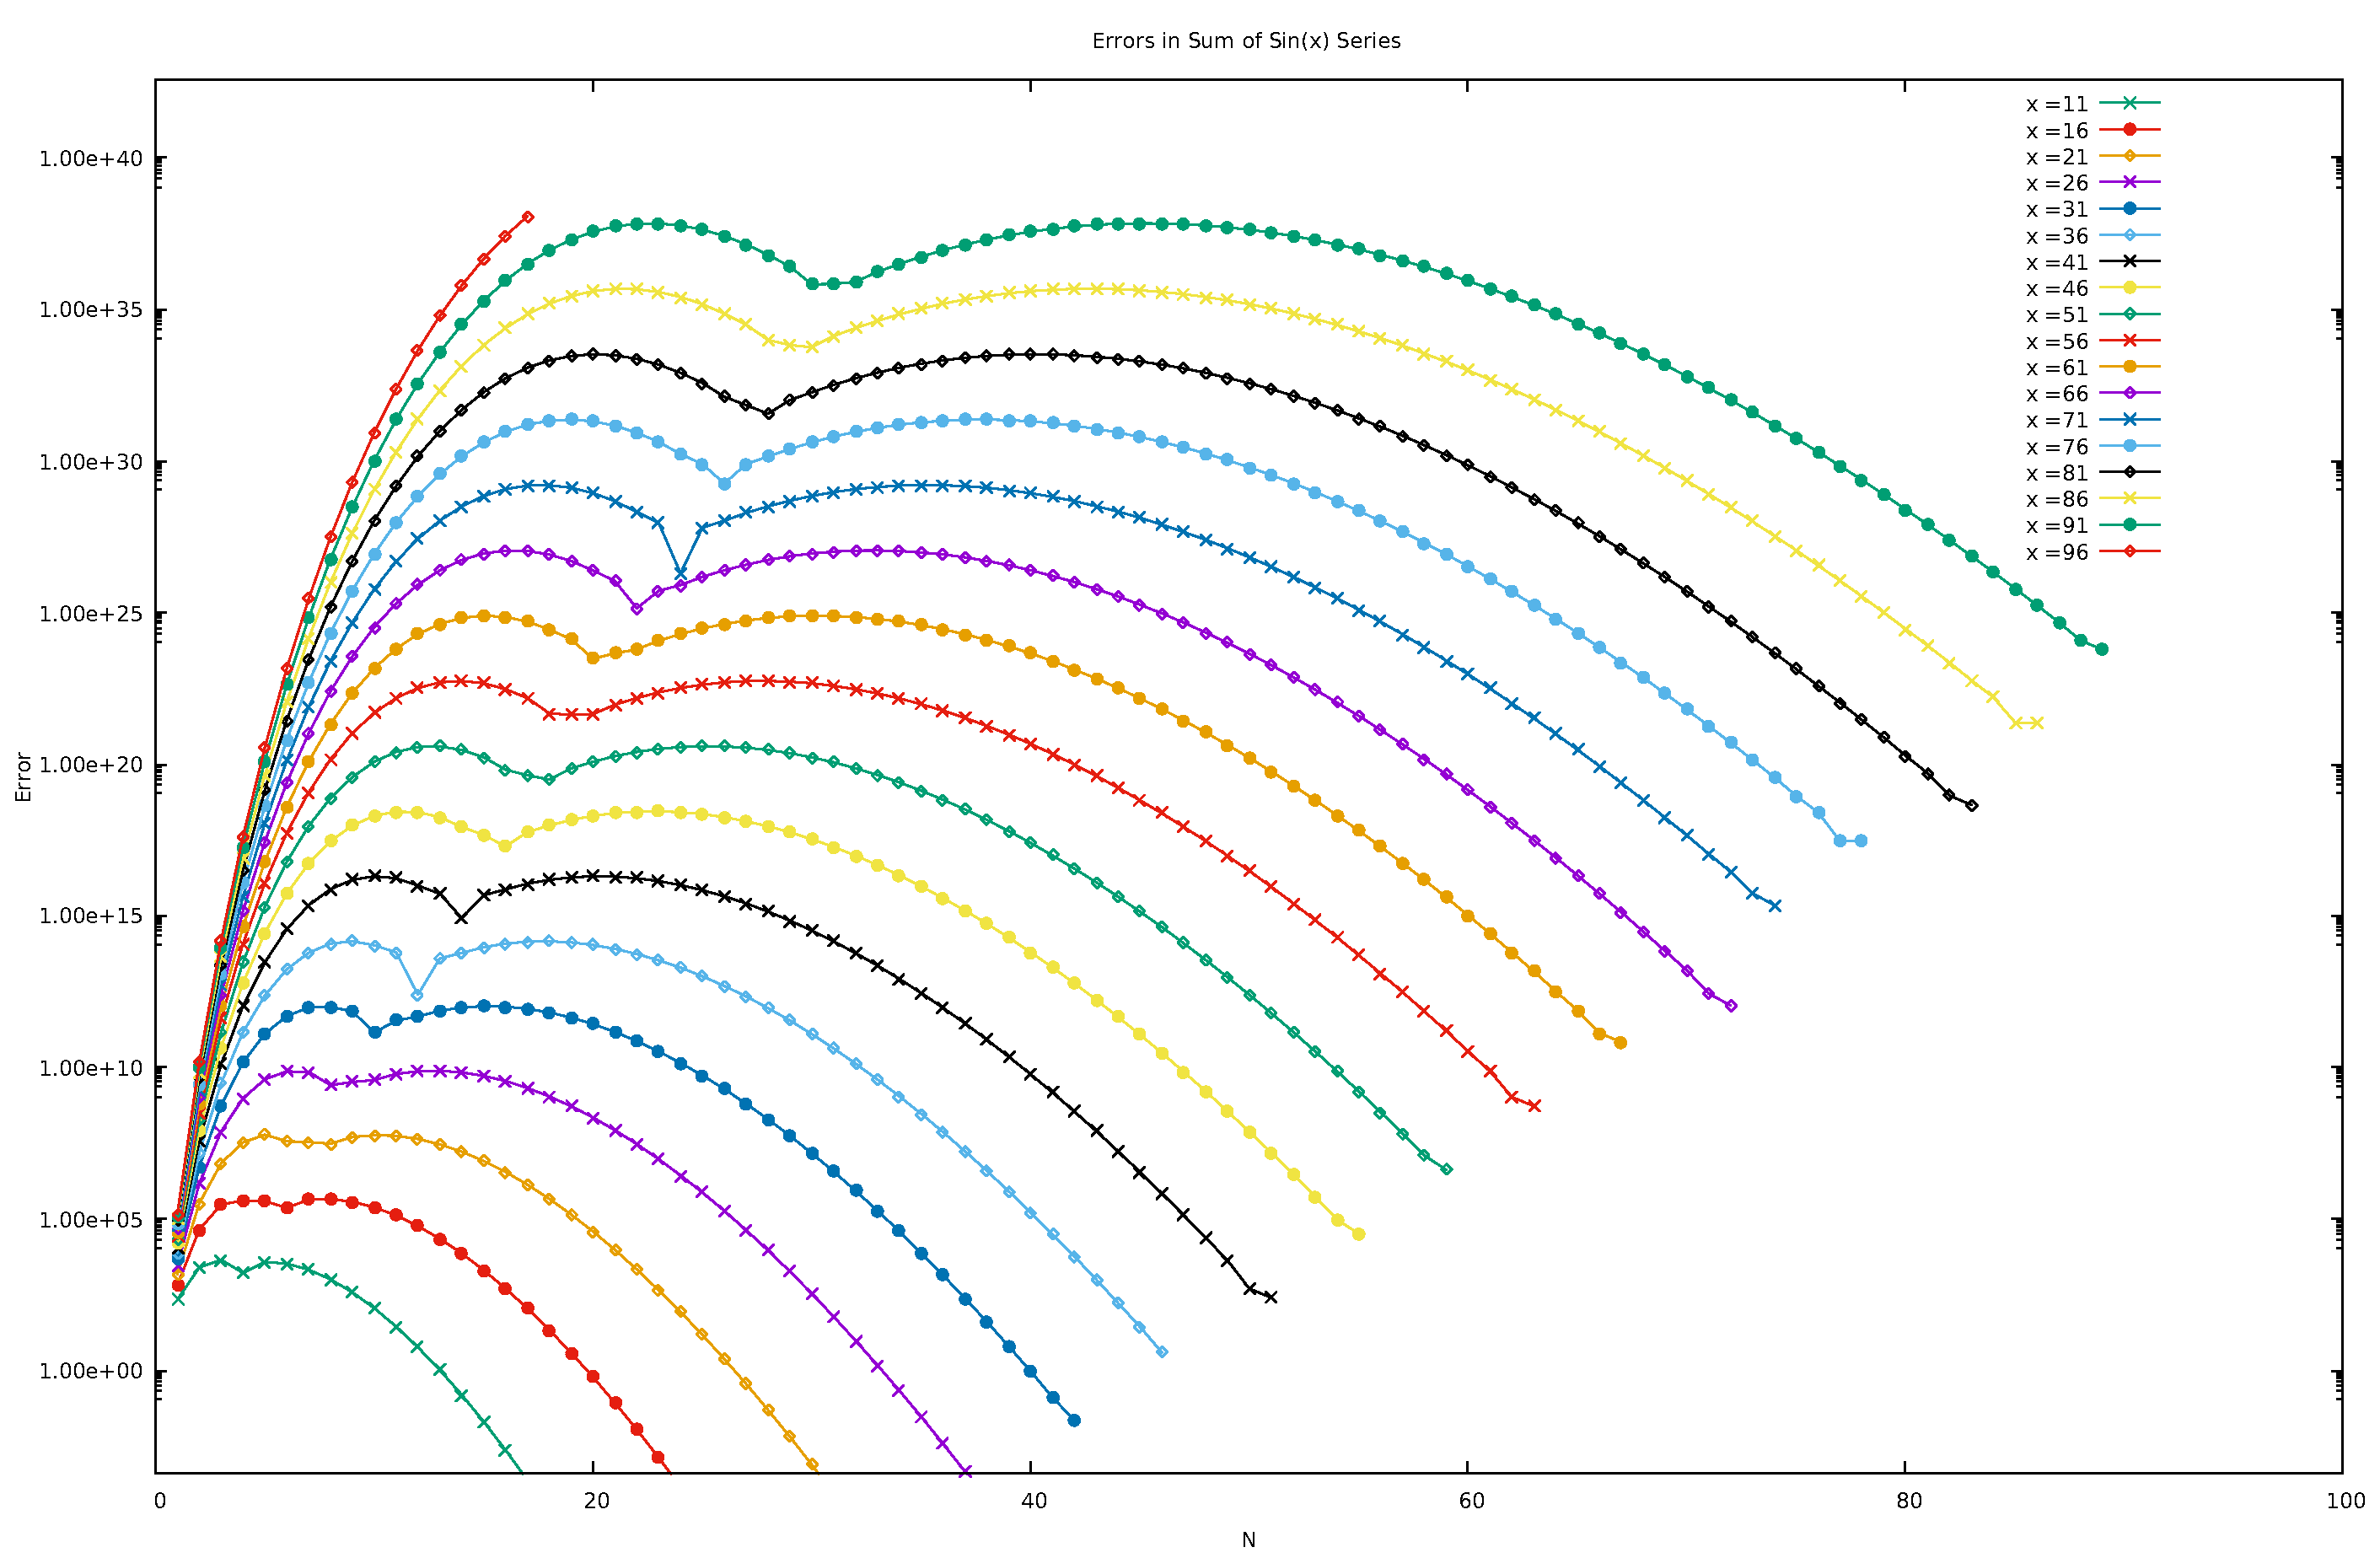
\includegraphics[scale=0.3]{/home/ishwarsingh/Phd_Documents/Course_work/Tutorial/Report/Images/sin_series_error_v2.pdf}
  \caption{Approximation errors in series sum of $\sin(x)$ for $10<x<100$.}
  \label{fig:sin_series_error2}
\end{figure}

\paragraph{Observations:}
  \begin{itemize}
    \item Note that the slope of the curve is negative for small values of $x$ i.e. the series converges for small values of x. Also there is no sharp dip in errors for small x which implies the absence of \emph{subtractive cancellation} in this range of $x$ values.
    \item The slope of the plot becomes positive after $x=5$ i.e. the errors increases with each computational step.
    \item Figure \ref{fig:sin_series_error2} shows that for very large values of $x$ the algorithm never converges
  \end{itemize}  




\section{Interaction of Errors in Computations}
Numerical algorithms play a pivotal role in modern simulations and calculations. However, it is important to study the convergence and precision of the algorithms chosen. In a traditional physics laboratory, true value of the physical quantity is generally known. This makes the calculations of errors and uncertainties a bit easier to compute. This however is not the case with most of the numerical algorithm. Then, the computation of errors or uncertainties gets tricky. Let us assume that an algorithm takes $N$ steps to complete, then the total error, $\epsilon_{t}$, in general, is given as,

\begin{align}
\epsilon_{t} &= \epsilon_{approx} + \epsilon_{ro} && \\
   \epsilon_{t}& = \frac{\alpha}{N^{\beta}} + \epsilon_m N^{\gamma}  &&  
\end{align}

\subsection{Implementation and Assessment}
To study the interaction of errors in scientific computation, consider a finite interaction of the following kind,

$$\int_{0}^{1} e^{-x}dx.$$
Analytically, we know that,

$$\int_{0}^{1} e^{-x}dx = 1-e^{-1} = 0.63212055.$$
Listing \ref{list6} lists a C++ code to calculate errors in Simpson's method of numerical integration. Figure \ref{fig:simpson} shows the variation of errors as a function of $N$ - the number of steps involved in the computation. 


\begin{lstlisting}[language=C++, caption= C++ code to calculate errors in Simpson's method of numerical integration., label= list6]
/*
 * Name - Ishwar Singh
 * Email  - isingh@fnal.gov
 * Date - 07.11.2020
 */

// CPP program for simpson's 1/3 rule 
#include <iostream> 
#include <fstream> 
#include <math.h> 
#include <iomanip> 
using namespace std; 
  
// Function to calculate f(x) 
float func(float x) 
{ 
    return exp(-x); 
} 
  
// Function for approximate integral 
float simpsons_(float ll, float ul, int n) 
{ 
    // Calculating the value of h 
    float h = (ul - ll) / n; 
  
    // Array for storing value of x and f(x) 
    float x[300], fx[300]; 
  
    // Calculating values of x and f(x) 
    for (int i = 0; i <= n; i++) { 
        x[i] = ll + i * h; 
        fx[i] = func(x[i]); 
    } 
  
    // Calculating result 
    float res = 0; 
    for (int i = 0; i <= n; i++) { 
        if (i == 0 || i == n) 
            res += fx[i]; 
        else if (i % 2 != 0) 
            res += 4 * fx[i]; 
        else
            res += 2 * fx[i]; 
    } 
    res = res * (h / 3); 
    return res; 
} 
  
// Driver program 
int main() 
{ 
    float lower_limit = 0; // Lower limit 
    float upper_limit = 1; // Upper limit 
    int n ; // Number of interval 
    std::ofstream my_file ;
    float true_val  = 0.63212055    ;
    my_file.open("simpson_v1.txt")  ;

    for(n=2;  n<=300;  n+=4){
    my_file <<  std::setprecision(7)<< n << "\t"  << abs((true_val - simpsons_(lower_limit, upper_limit, n))/true_val)  <<  std::endl; 
    }
    return 0; 
} 
\end{lstlisting} 


\begin{figure}[h]
    \centering
    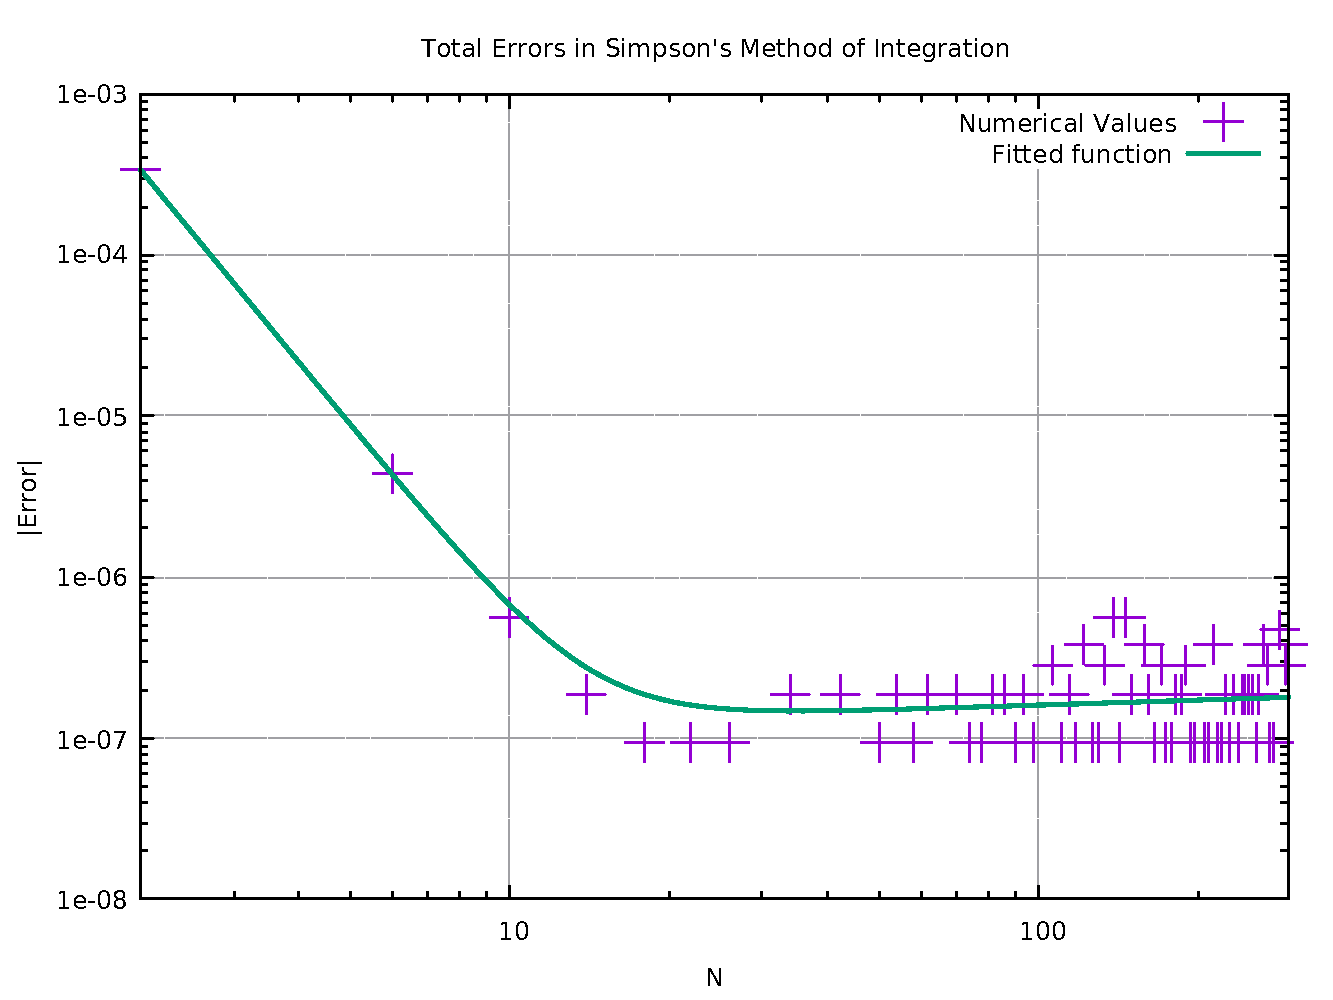
\includegraphics[scale=0.5]{/home/ishwarsingh/Phd_Documents/Course_work/Tutorial/Report/Images/simpson.pdf}
  \caption{Errors in Simpson's rule of numerical integration.}
  \label{fig:simpson}
\end{figure}

\subsubsection{Observations}
  \begin{itemize}
    \item Observe the rapid decrease in the errors for smaller $N$ values. This is a characteristics of \emph{approximation errors} which varies as $\propto\frac{\alpha}{N^{\beta}}$ with $\beta>0$.
    \item As the value of $N$ increases, a slow, irregular increase is observed. This is because of the fact that, in general, the \emph{round-off errors} varies as $\propto N^{\gamma}$, with $\gamma>0$.
    \item This curve gives an \emph{optimized value of the number of iterations} to stop the algorithm.

  \end{itemize}  

  \section{Conclusions}
  It can now be concluded that every scientific computation is prone to errors and uncertainties similar to a measurement in a traditional physics laboratory. These errors propagate at each computation step which might lead to a \emph{garbage value}, which of-course is of no use. As the role of numerical computation is becoming more and more pivotal, the subtleties of these errors must be emphasized. It will be a total waste of huge computing powers if the result is a garbage value. Therefore, it is important to analyze the role of each and every source of errors in scientific computation before actually jumping to trust their results.  \nocite{landau2008survey} \nocite{fadnavis1998some} \nocite{goldberg1991every} \nocite{numeric_ana_1} \nocite{fpc} \nocite{Keinert}
\pagebreak
\printbibliography
\end{document}
